\documentclass[11pt]{article}
\usepackage[margin=0.75in]{geometry}
\usepackage{amsmath,amssymb}
\usepackage{xcolor}
\usepackage{tikz}
\usepackage[most]{tcolorbox}
\usepackage{enumitem}
\usepackage{titlesec}
\usepackage{fancyhdr}

\definecolor{ink}{HTML}{1F3A5F}
\definecolor{key}{HTML}{8A1C1C}
\definecolor{soft}{HTML}{EEF3F8}
\definecolor{warm}{HTML}{FBF3E6}

\setlength{\parindent}{0pt}
\setlength{\parskip}{4pt}
\setlist{itemsep=1pt,topsep=2pt}
\titleformat{\section}{\large\bfseries\color{ink}}{\thesection.}{0.5em}{}
\titleformat{\subsection}{\normalsize\bfseries\color{ink}}{}{0em}{}
\titlespacing*{\section}{0pt}{10pt}{4pt}
\titlespacing*{\subsection}{0pt}{6pt}{2pt}

\newcommand{\E}{\mathrm{E}}

\newtcolorbox{bigidea}{colback=soft,colframe=ink,boxrule=0.6pt,arc=2pt,left=5pt,right=5pt,top=3pt,bottom=3pt,
  title={\bfseries\small Big idea},fonttitle=\small}
\newtcolorbox{trap}{colback=warm,colframe=key,boxrule=0.6pt,arc=2pt,left=5pt,right=5pt,top=3pt,bottom=3pt,
  title={\bfseries\small Traps / what graders look for},fonttitle=\small}
\newtcolorbox{answer}{colback=white,colframe=ink,boxrule=0.6pt,arc=2pt,left=6pt,right=6pt,top=4pt,bottom=4pt,
  title={\bfseries\small Model answer},fonttitle=\small,breakable}

\pagestyle{fancy}
\fancyhf{}
\renewcommand{\headrulewidth}{0pt}
\fancyfoot[C]{\small\thepage}

% Shared TikZ figures for the ECON 5040 midterm study guide and sample midterm.
% Each \fig... macro draws one self-contained tikzpicture.

% 1. Intertemporal budget line: R is minus the slope
\newcommand{\figIntertemporal}{%
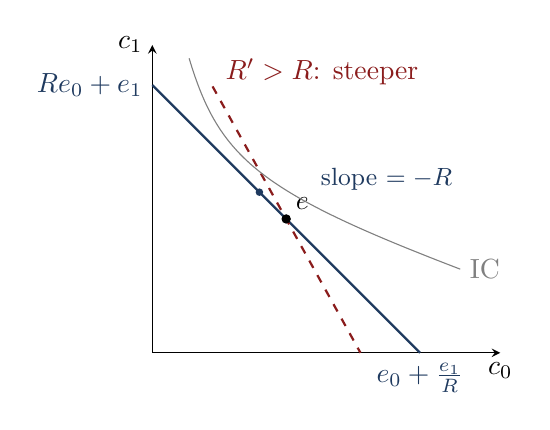
\begin{tikzpicture}[scale=0.85,>=stealth]
  \draw[->] (0,0) -- (5.2,0) node[below] {$c_0$};
  \draw[->] (0,0) -- (0,4.6) node[left] {$c_1$};
  % endowment e = (2,2); budget with R = 1 (slope -1) and R' > R (slope -1.8)
  \draw[thick,ink] (0,4) -- (4,0) node[below] {$e_0+\tfrac{e_1}{R}$};
  \node[left,ink] at (0,4) {$Re_0+e_1$};
  \draw[thick,key,dashed] (0.9,3.98) -- (3.11,0);
  \node[key,right] at (0.95,4.2) {$R'>R$: steeper};
  \fill (2,2) circle (2pt) node[above right] {$e$};
  % indifference curve tangent to the original line at (1.6,2.4)
  \draw[gray] (0.55,4.4) .. controls (1.0,2.9) and (1.6,2.4) .. (4.6,1.25);
  \fill[ink] (1.6,2.4) circle (1.6pt);
  \node[gray,right] at (4.6,1.25) {IC};
  \node[ink] at (3.5,2.6) {\small slope $=-R$};
\end{tikzpicture}}

% 2. Concave utility, expected utility, certainty equivalent
\newcommand{\figCE}{%
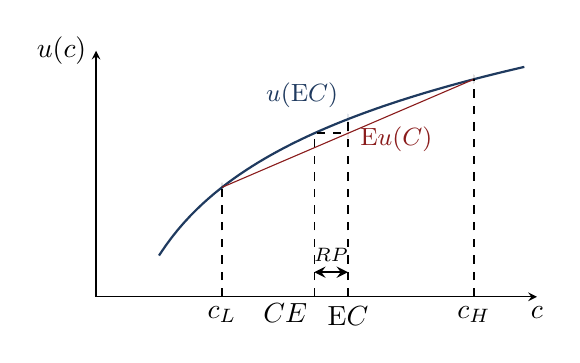
\begin{tikzpicture}[xscale=0.032,yscale=1.25,>=stealth]
  \draw[->] (0,2.8) -- (175,2.8) node[below] {$c$};
  \draw[->] (0,2.8) -- (0,5.3) node[left] {$u(c)$};
  \draw[thick,ink,domain=25:170,samples=60] plot (\x,{ln(\x)});
  \draw[key] (50,{ln(50)}) -- (150,{ln(150)});
  \fill (50,{ln(50)}) circle (1.4pt); \fill (150,{ln(150)}) circle (1.4pt);
  % E[C]=100, E[u]=0.5(ln50+ln150)=4.4637, CE=86.6, u(100)=4.6052
  \fill[key] (100,4.4637) circle (1.6pt);
  \fill[ink] (100,4.6052) circle (1.6pt);
  \draw[dashed] (100,2.8) node[below] {$\E C$} -- (100,4.6052);
  \draw[dashed] (86.6,2.8) node[below left=-1pt] {$CE$} -- (86.6,4.4637) -- (100,4.4637);
  \draw[dashed] (50,2.8) node[below] {$c_L$} -- (50,{ln(50)});
  \draw[dashed] (150,2.8) node[below] {$c_H$} -- (150,{ln(150)});
  \node[ink,above left] at (100,4.62) {\small $u(\E C)$};
  \node[key,right] at (101,4.40) {\small $\E u(C)$};
  \draw[<->,thick] (86.6,3.05) -- node[above] {\scriptsize $RP$} (100,3.05);
\end{tikzpicture}}

% 3. Two-state Markov chain
\newcommand{\figMarkov}{%
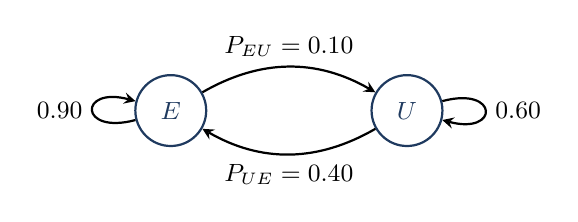
\begin{tikzpicture}[>=stealth,node distance=3cm,every node/.style={font=\small}]
  \node[circle,draw,thick,ink,minimum size=9mm] (E) {$E$};
  \node[circle,draw,thick,ink,minimum size=9mm,right of=E] (U) {$U$};
  \draw[->,thick] (E) to[bend left] node[above] {$P_{EU}=0.10$} (U);
  \draw[->,thick] (U) to[bend left] node[below] {$P_{UE}=0.40$} (E);
  \draw[->,thick] (E) to[loop left] node[left] {$0.90$} (E);
  \draw[->,thick] (U) to[loop right] node[right] {$0.60$} (U);
\end{tikzpicture}}

% 4. Bellman decomposition / timing
\newcommand{\figBellman}{%
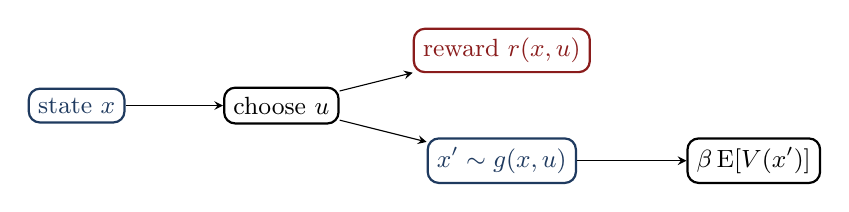
\begin{tikzpicture}[>=stealth,every node/.style={font=\small}]
  \node[draw,rounded corners,ink,thick] (x) at (0,0) {state $x$};
  \node[draw,rounded corners,thick] (u) at (2.6,0) {choose $u$};
  \node[draw,rounded corners,key,thick] (r) at (5.4,0.7) {reward $r(x,u)$};
  \node[draw,rounded corners,ink,thick] (xp) at (5.4,-0.7) {$x'\sim g(x,u)$};
  \node[draw,rounded corners,thick] (v) at (8.6,-0.7) {$\beta\,\E[V(x')]$};
  \draw[->] (x) -- (u); \draw[->] (u) -- (r); \draw[->] (u) -- (xp); \draw[->] (xp) -- (v);
\end{tikzpicture}}

% 5. Solow: sf(k) vs delta k, with a rise in s
\newcommand{\figSolow}{%
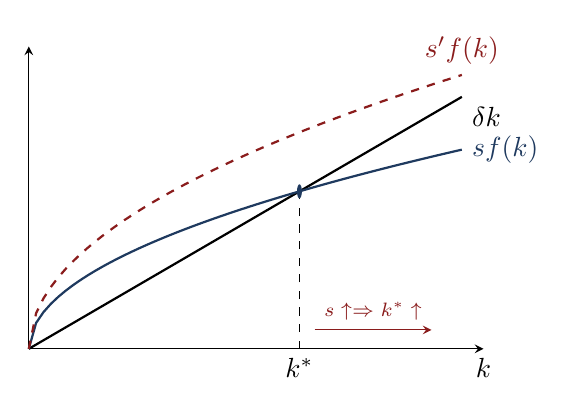
\begin{tikzpicture}[xscale=0.55,yscale=1.6,>=stealth]
  \draw[->] (0,0) -- (10.5,0) node[below] {$k$};
  \draw[->] (0,0) -- (0,2.4);
  \draw[thick] (0,0) -- (10,2) node[below right] {$\delta k$};
  \draw[thick,ink,domain=0:10,samples=60] plot (\x,{0.4*sqrt(\x)*1.25}) node[right] {$sf(k)$};
  \draw[thick,key,dashed,domain=0:10,samples=60] plot (\x,{0.55*sqrt(\x)*1.25}) node[above] {$s'f(k)$};
  % k* where 0.5 sqrt k = 0.2 k -> k = 6.25 ; k*' where 0.6875 sqrt k = 0.2k -> k = 11.8 (off-axis) so use 0.55*1.25=0.6875
  \draw[dashed] (6.25,0) node[below] {$k^*$} -- (6.25,1.25);
  \fill[ink] (6.25,1.25) circle (1.6pt);
  \draw[->,key] (6.6,0.15) -- (9.3,0.15) node[midway,above] {\scriptsize $s\uparrow\Rightarrow k^*\uparrow$};
  
\end{tikzpicture}}

% 6. Level effect vs growth effect
\newcommand{\figLevelGrowth}{%
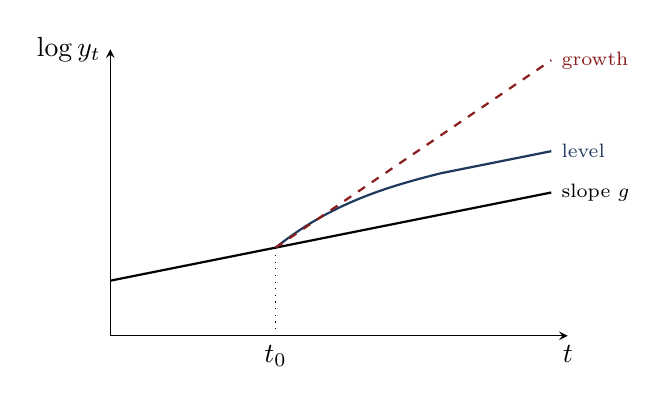
\begin{tikzpicture}[xscale=0.7,yscale=0.7,>=stealth]
  \draw[->] (0,0) -- (8.3,0) node[below] {$t$};
  \draw[->] (0,0) -- (0,5.2) node[left] {$\log y_t$};
  \draw[thick] (0,1) -- (8,2.6) node[right] {\scriptsize slope $g$};
  \draw[thick,ink] (3,1.6) .. controls (4,2.4) and (5,2.7) .. (6,2.95) -- (8,3.35) node[right] {\scriptsize level};
  \draw[thick,key,dashed] (3,1.6) -- (8,5.0) node[right] {\scriptsize growth};
  \draw[dotted] (3,0) node[below] {$t_0$} -- (3,1.6);
\end{tikzpicture}}

% 7. Convex marginal utility -> precautionary saving
\newcommand{\figPrecaution}{%
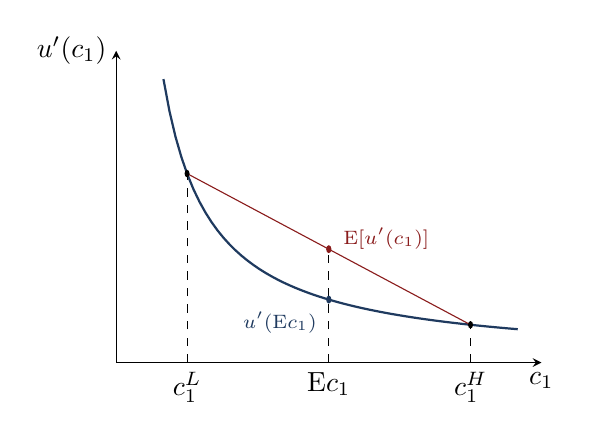
\begin{tikzpicture}[xscale=0.6,yscale=0.9,>=stealth]
  \draw[->] (0,0) -- (9,0) node[below] {$c_1$};
  \draw[->] (0,0) -- (0,4.4) node[left] {$u'(c_1)$};
  \draw[thick,ink,domain=1:8.5,samples=60] plot (\x,{4/\x});
  \draw[key] (1.5,2.667) -- (7.5,0.533);
  \fill (1.5,2.667) circle (1.5pt); \fill (7.5,0.533) circle (1.5pt);
  \draw[dashed] (1.5,0) node[below] {$c_1^L$} -- (1.5,2.667);
  \draw[dashed] (7.5,0) node[below] {$c_1^H$} -- (7.5,0.533);
  \draw[dashed] (4.5,0) node[below] {$\E c_1$} -- (4.5,1.6);
  \fill[key] (4.5,1.6) circle (1.6pt); \fill[ink] (4.5,0.889) circle (1.6pt);
  \node[key,right] at (4.6,1.75) {\scriptsize $\E[u'(c_1)]$};
  \node[ink,below left] at (4.45,0.85) {\scriptsize $u'(\E c_1)$};
\end{tikzpicture}}

% 8. McCall reservation wage
\newcommand{\figMcCall}{%
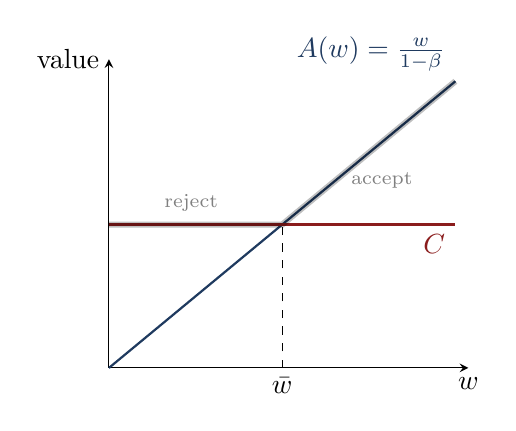
\begin{tikzpicture}[xscale=0.55,yscale=0.7,>=stealth]
  \draw[->] (0,0) -- (8.3,0) node[below] {$w$};
  \draw[->] (0,0) -- (0,5.6) node[left] {value};
  \draw[thick,ink] (0,0) -- (8,5.2) node[above left] {$A(w)=\frac{w}{1-\beta}$};
  \draw[thick,key] (0,2.6) -- (8,2.6) node[below left] {$C$};
  \draw[dashed] (4,0) node[below] {$\bar w$} -- (4,2.6);
  \draw[line width=2.2pt,opacity=0.25] (0,2.6) -- (4,2.6) -- (8,5.2);
  \node[gray] at (1.9,3.0) {\scriptsize reject};
  \node[gray] at (6.3,3.4) {\scriptsize accept};
\end{tikzpicture}}


\newcounter{qn}
\newcommand{\question}[1]{\refstepcounter{qn}\par\medskip
{\bfseries\color{ink}Question \theqn.\ #1}\par\smallskip}

\begin{document}

\begin{center}
{\LARGE\bfseries\color{ink} ECON 5040 Sample Midterm, with Model Answers}\\[3pt]
{\small Closed book, closed notes. Ten questions, one per study-guide topic. Answer each in a short paragraph (3--4 sentences); a graph may help.\\
The questions follow the official study guide's bullets closely. Each model answer is written to earn a 10/10: idea, equation, mechanism, graph.}
\end{center}

\question{Inter-temporal prices}
Explain how the real interest rate determines the relative price of consumption today and consumption in the future. Then explain the substitution incentive created by an increase in the real interest rate.

\begin{answer}
\begin{minipage}[t]{0.56\textwidth}\vspace{0pt}
Consumption today and consumption next period are different commodities, and the gross real interest rate $R=1+r$ is their relative price. Giving up one unit of $c_0$ buys $R$ units of $c_1$, so the price of future consumption in today's units is $1/R$ and the intertemporal budget line $c_0+c_1/R=e_0+e_1/R$ has slope $-R$. At an optimum the household sets its MRS equal to this price: $u'(c_0)/[\beta u'(c_1)]=R$. When $R$ rises, future consumption becomes cheaper relative to current consumption (the budget line pivots through the endowment and steepens). The \textbf{substitution effect} therefore always pushes the household to consume less today and save more. The total effect can be offset by an income effect for lenders, who become richer when $R$ rises.
\end{minipage}\hfill
\begin{minipage}[t]{0.4\textwidth}\vspace{0pt}\centering
\figIntertemporal
\end{minipage}
\end{answer}

\question{Choice under uncertainty}
A consumer with $u(c)=\log c$ faces a gamble paying $c=50$ or $c=150$ with equal probability. Compute and interpret the certainty equivalent, and explain how the curvature of $u$ affects the value of this risky prospect.

\begin{answer}
\begin{minipage}[t]{0.56\textwidth}\vspace{0pt}
Under expected utility the gamble is worth $\E u(C)=\tfrac12\log50+\tfrac12\log150$. The certainty equivalent solves $u(CE)=\E u(C)$, so $CE=\exp(\tfrac12\log50+\tfrac12\log150)=\sqrt{7500}\approx\mathbf{86.60}$. The consumer is indifferent between the gamble and 86.60 for sure, even though $\E C=100$, so the risk premium is $100-86.60=13.40$. This happens because $\log$ is concave: diminishing marginal utility makes the loss from the bad outcome hurt more than the equal gain from the good outcome helps. Jensen's inequality then gives $\E u(C)<u(\E C)$. The more curved $u$ is (higher $\rho=-cu''/u'$), the lower the $CE$ and the larger the risk premium; a risk-neutral consumer (linear $u$) would value the gamble at $\E C=100$.
\end{minipage}\hfill
\begin{minipage}[t]{0.4\textwidth}\vspace{0pt}\centering
\figCE
\end{minipage}
\end{answer}

\question{Markov processes}
State the Markov property. For a worker whose status follows $P=\begin{bmatrix}0.90&0.10\\0.40&0.60\end{bmatrix}$ (state 1 = employed, state 2 = unemployed), interpret the element $P_{21}$ and the first row of $P$.

\begin{answer}
\begin{minipage}[t]{0.6\textwidth}\vspace{0pt}
A process is Markov if, conditional on the current state, the past gives no additional information about the distribution of the next state: $\Pr(X_{t+1}=j\mid X_t=i,X_{t-1},\dots)=\Pr(X_{t+1}=j\mid X_t=i)$. History can still matter, but only through the state it produced. Element $P_{ij}=\Pr(X_{t+1}=j\mid X_t=i)$, so $P_{21}=0.40$ is the probability that a worker unemployed today is employed next period: the \textbf{job-finding rate}. The first row $(0.90,\,0.10)$ is the entire conditional distribution of tomorrow's status for someone employed today: a 90\% chance of keeping the job and a 10\% separation rate. Each row is non-negative and sums to one. The population distribution evolves as $\psi_{t+1}=\psi_tP$, with stationary distribution $\psi^*=(0.8,0.2)$.
\end{minipage}\hfill
\begin{minipage}[t]{0.36\textwidth}\vspace{6pt}\centering
\figMarkov
\end{minipage}
\end{answer}

\question{Introduction to dynamic programming}
Write the Bellman equation and explain how it decomposes a dynamic problem. For the optimal growth problem ($c_t+k_{t+1}=Ak_t^\alpha$, utility $\sum\beta^t\log c_t$), identify the state variable, choice variable, current payoff, and next-period state.

\begin{answer}
The Bellman equation is $V(x)=\max_{u}\{r(x,u)+\beta\,\E[V(x')\mid x,u]\}$ with $x'\sim g(x,u)$. It turns an infinite-horizon sequence problem into a choice of one action today. That action is valued as the \textbf{current reward} $r(x,u)$ plus the \textbf{discounted expected continuation value} of the state it leads to, where $V$ already embodies optimal behavior from tomorrow on. The control can matter in both places: through today's reward and through the distribution of tomorrow's state. In the growth model the \textbf{state} is current capital $k_t$, the \textbf{choice} is next period's capital $k_{t+1}$ (equivalently $c_t$), the \textbf{current payoff} is $\log(Ak_t^\alpha-k_{t+1})$, and the \textbf{next state} is $k'=k_{t+1}$. So $V(k)=\max_{k'}\{\log(Ak^\alpha-k')+\beta V(k')\}$, whose solution is the policy $k'=\alpha\beta Ak^\alpha$.
\end{answer}

\question{Value functions and policy functions}
Distinguish the value function from the policy function. What economic information does each provide, and how is the optimal policy related to the Bellman equation?

\begin{answer}
The \textbf{value function} $V(x)$ answers ``how good is it to be in state $x$, knowing I will behave optimally from now on?'' It is the maximized expected discounted lifetime payoff, a number for each state. The \textbf{policy function} $h(x)$ answers ``what should I do in state $x$?'' It is a contingent plan assigning an action to every state, which is what a solution must be when future states are random. $V$ provides welfare and shadow values (e.g.\ $V'(x)=u'(c)$ is the value of one more unit of wealth), while $h$ provides behavior: the saving rule, the reservation-wage rule, and the law of motion $x_{t+1}\sim g(x_t,h(x_t))$. The two are linked by the Bellman equation: $h(x)=\arg\max_u\{r(x,u)+\beta\E[V(x')\mid x,u]\}$, and $V$ is the value of following $h$ forever. For example, in McCall $V(w)=\max\{w/(1-\beta),C\}$, while the policy is ``accept iff $w\ge\bar w$.''
\end{answer}

\question{Howard's method versus value function iteration}
Explain the logic of value function iteration and of Howard's policy-improvement method. Why can Howard's method be much faster?

\begin{answer}
\textbf{Value function iteration} starts with a guess $V_0$ (e.g.\ zeros) and repeatedly applies the Bellman operator $V_{n+1}(x)=\max_u\{r(x,u)+\beta\sum_{x'}M_u(x,x')V_n(x')\}$. Each step adds one more period of future rewards. It stops when $V$ stops changing and then reads off $h=\arg\max$; since $T$ is a contraction with modulus $\beta$, the error shrinks only by about a factor $\beta$ per step, which is slow when $\beta$ is near 1. \textbf{Howard's method} starts with a guessed \emph{policy} and separates two steps. \emph{Policy evaluation:} with the policy fixed the max disappears, so solve the linear system $V_h=(I-\beta P_h)^{-1}r_h$ for the exact value of following $h$ forever. \emph{Policy improvement:} choose the best action in each state given $V_h$; stop when the policy no longer changes. It is faster because each evaluation does in one linear solve what VFI would need infinitely many iterations to do. Since there are finitely many policies and each round improves, it typically converges in just a few iterations.
\end{answer}

\question{The Solow model}
Explain how saving and capital accumulation determine steady-state capital and output in the Solow model. Does a permanent increase in the saving rate permanently raise the growth rate of output per worker?

\begin{answer}
\begin{minipage}[t]{0.54\textwidth}\vspace{0pt}
With an exogenous saving rate $s$, capital per worker evolves as $k_{t+1}=sf(k_t)+(1-\delta)k_t$. Because $f$ has diminishing returns, investment $sf(k)$ exceeds depreciation $\delta k$ at low $k$ (capital grows) and falls short at high $k$ (capital shrinks). The economy therefore converges to the steady state $sf(k^*)=\delta k^*$; with Cobb--Douglas, $k^*=(sA/\delta)^{1/(1-\alpha)}$ and $y^*=A(k^*)^\alpha$. A permanent rise in $s$ shifts $sf(k)$ up, raising $k^*$ and $y^*$: a \textbf{level effect}. Growth is faster only temporarily, during the transition. It does \emph{not} permanently raise growth, because diminishing returns mean the extra capital eventually only covers depreciation. Long-run growth of output per worker equals the rate of technological progress $g$, which is exogenous in Solow.
\end{minipage}\hfill
\begin{minipage}[t]{0.43\textwidth}\vspace{0pt}\centering
\figSolow\\[4pt]
\figLevelGrowth
\end{minipage}
\end{answer}

\question{Optimal saving}
Interpret the Euler equation $u'(c_t)=\beta R\,\E_t[u'(c_{t+1})]$. How does a household adjust if $u'(c_t)>\beta R\,\E_t[u'(c_{t+1})]$?

\begin{answer}
The left side is the marginal utility of consuming one more unit today. The right side is the value of saving that unit instead: it grows to $R$ units tomorrow, each worth $u'(c_{t+1})$ in expectation, discounted by $\beta$. At an optimum the household is indifferent at the margin, so the two must be equal; this holds every period along the optimal path (MRS $=R$). If $u'(c_t)>\beta R\E_tu'(c_{t+1})$, a unit consumed today is worth more than the same unit saved, so the household should \textbf{consume more today and save less}. Doing so lowers $u'(c_t)$ and, because $c_{t+1}$ falls, raises $u'(c_{t+1})$, until the equation holds. (In the opposite case it saves more.) The only exception is a binding borrowing constraint: then the household wants to consume more but cannot, and the strict inequality persists.
\end{answer}

\question{Income fluctuations}
Explain why uncertainty about future income can increase saving even when expected future income is unchanged, and why assets provide self-insurance.

\begin{answer}
\begin{minipage}[t]{0.56\textwidth}\vspace{0pt}
Saving is set by $u'(c_0)=\beta R\E[u'(c_1)]$. When marginal utility is convex ($u'''>0$, as with log or CRRA utility), Jensen's inequality implies $\E[u'(c_1)]>u'(\E c_1)$. A mean-preserving spread in future income therefore raises the expected marginal value of saving at every asset level, so the household saves more. This is \textbf{precautionary saving}, and it happens even though expected income is unchanged. Economically, low-income states have very high marginal utility, so a dollar carried into them is especially valuable. The asset pays $R$ in every state, so it is not insurance, but consumption is chosen after income is observed: the household runs down its buffer when income is low. That transfers resources toward the future states where consumption and wealth are low, which is \textbf{self-insurance} when insurance markets are incomplete.
\end{minipage}\hfill
\begin{minipage}[t]{0.4\textwidth}\vspace{0pt}\centering
\figPrecaution
\end{minipage}
\end{answer}

\question{Putting the ideas together: job search}
Explain why job search is a dynamic decision problem. Formulate the McCall problem in terms of the state variable, choice variable, transition, and continuation value, and explain the reservation wage.

\begin{answer}
\begin{minipage}[t]{0.56\textwidth}\vspace{0pt}
Job search is dynamic because rejecting an offer affects both today's payoff (unemployment benefit $c$ instead of $w$) and tomorrow's opportunities (the chance to draw a better offer). Accepting ends the search forever, so it is an \textbf{optimal stopping} problem. The \textbf{state} is the current offer $w$, the \textbf{choice} is accept or reject, and the \textbf{transition} is: accept means you earn $w$ forever, reject means a new offer $W'\sim F$ (IID) next period. The Bellman equation is $V(w)=\max\{w/(1-\beta),\ c+\beta\E V(W')\}$, where the \textbf{continuation value} $C=c+\beta\E V(W')$ is the value of not stopping yet and keeping the option to choose again. Since $A(w)=w/(1-\beta)$ rises with $w$ while $C$ is constant (offers are IID), there is a \textbf{reservation wage} $\bar w=(1-\beta)C$: accept iff $w\ge\bar w$. Higher $c$ or higher $\beta$ raises $\bar w$.
\end{minipage}\hfill
\begin{minipage}[t]{0.4\textwidth}\vspace{0pt}\centering
\figMcCall
\end{minipage}
\end{answer}

\end{document}
